%Sensorthing<SensorthingT> 
\rule{\textwidth}{0.4pt}
\class{Sensorthing<SensorthingT>}
\begin{minipage}{0.4\textwidth}
    \begin{figure}[H]
        {\centering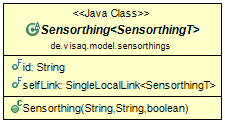
\includegraphics[width=0.95\textwidth]{media/backend/modell/classes/Sensorthing.png}}
    \end{figure}
    \end{minipage} \hfill
    \begin{minipage}{0.6\textwidth}
Die abstrakte Klasse Sensorthing stellt ein Objekt aus der \gls{SensorThings API} da.
Die Klasse vereint die gemeinsamen Eigenschaften der Klassen aus der Datenbank-\gls{API} in sich.
Um die Datentypen der Parameter möglichst exakt zu bestimmen werden \glspl{f-bounded quantification} verwendet.
\end{minipage}

Attribute:
\begin{itemize}
    \item \emph{public String id} Jedes Objekt der Datenbank-\gls{API} ist mit einer eindeutigen ID versehen, die das Objekt identifiziert.
    Da sich die ID aus Buchstaben, Zeichen und Ziffern zusammensetzt wird sie hier durch einen String repräsentiert.
    \item \emph{public SingleLocalLink<SensorthingT> selfLink} Jedes Objekt der \gls{SensorThings API} hält einen Verweis auf die Online-Instanz von sich selbst.
    So kann die Herkunft und die übereinstimmung des Datensatzes mit der Online-Version jederzeit überprüft werden.
\end{itemize}
Methoden: \begin{itemize}
    \item \emph{public Sensorthing(String id, String selfURL, boolean relative)} Diese Methode ist er einzige Konstruktor der Sensorthing-Klasse.
    Als Parameter erhält der Konstruktor neben dem Klassen-Attribut id auch eine URL und eine boolean relative. Beide Parameter werden zum initialisieren des SingleLocalLink benötigt.
\end{itemize}

%Datastream